\documentclass[11pt]{article}

\usepackage[a4paper,margin=1in]{geometry}
\usepackage[T1]{fontenc}
\usepackage{lmodern}
\usepackage{microtype}
\usepackage{amsmath,amssymb,amsthm,mathtools}
\usepackage{booktabs}
\usepackage{graphicx}
\usepackage{xcolor}
\usepackage{enumitem}
\usepackage{caption}
\usepackage{hyperref}

\hypersetup{
  colorlinks=true,
  linkcolor=cyan!45!black,
  citecolor=magenta!70!black,
  urlcolor=cyan!45!black
}

\newtheorem{assumption}{Assumption}
\newtheorem{proposition}{Proposition}
\newtheorem{remark}{Remark}
\newcommand{\eps}{\varepsilon}
\newcommand{\Bin}{\operatorname{Bin}}
\newcommand{\Prob}{\Pr}
\newcommand{\ceilodd}[1]{\left\lceil #1 \right\rceil_{\mathrm{odd}}}

\title{Performance- and Cost-Driven Benchmarking\\
under i.i.d. Circuit-Level Noise}
\author{Technical note for an analog quantum-computing project}
\date{\today}

\begin{document}
\maketitle

\begin{abstract}
This note reformulates the repetition and majority-vote analysis of
trap-based verification as a benchmarking procedure under an independent and
identically distributed (i.i.d.) circuit-level noise assumption. Test rounds
are first used to infer an upper confidence bound on the noise rate of a fixed
circuit instance. This bound is then converted into an upper bound on the
probability that one computation round returns the wrong decision bit. Two
complementary benchmarks follow: a performance-driven benchmark, which returns
the number of computation rounds required to reach a fixed correctness error,
and a cost-driven benchmark, which returns the correctness error reached with
a fixed number of computation rounds. The specialization to two test types,
$k=2$, explains the conservative $1/4$ test-failure threshold when the ideal
computation error is negligible.
\end{abstract}

\section{Scope and relation to verification}

The verification protocol of Sater and Ollivier uses $d$ computation rounds,
$s$ test rounds, a rejection threshold $w$, and $k$ trap types. Its correctness
proof bounds the error of a majority vote, while its security proof treats an
arbitrary malicious deviation and maximizes over the worst deviation. Its
robustness statement accepts an honest noisy device when the circuit-level
noise rate is below $w/s$; security requires $w/s<\alpha/k$, where
\begin{equation}
  \alpha=\frac{1-2c}{2-2c},
  \label{eq:alpha}
\end{equation}
and $c<1/2$ is the intrinsic error of one ideal computation round
\cite{sater2026magicblindness}.

The present analysis makes a stronger physical assumption and obtains a weaker
cryptographic conclusion. The device is assumed to apply the same unknown noise
process independently on every round of a fixed circuit. Under this model, all
test rounds may be executed as one benchmarking block. The benchmark estimates
a stationary noise parameter, and the resulting estimate is used to size a
subsequent majority vote. This is not a composable verification guarantee
against a malicious or drifting device.

\section{Assumptions}

Fix a circuit instance, possibly indexed by a circuit dimension $\ell$.

\begin{assumption}[i.i.d. rounds]
For a fixed circuit instance $\ell$, every test and computation round is an
independent sample from the same stationary device behavior.
\end{assumption}

\begin{assumption}[Transfer from tests to computations]
A harmful round is detected by a uniformly selected test type with probability
at least $1/k$. Equivalently, if $r_\ell$ is the harmful-round probability and
$q_\ell$ is the average test-failure probability, then
\begin{equation}
  q_\ell \ge \frac{r_\ell}{k},
  \qquad\text{hence}\qquad
  r_\ell\le kq_\ell.
  \label{eq:test-to-harmful}
\end{equation}
\end{assumption}

\begin{assumption}[Worst-case effect of a harmful round]
An unaffected computation round is wrong with probability at most $c_\ell$,
whereas a harmful round may be wrong with probability one.
\end{assumption}

Assumption 2 is the conservative bridge inherited from the trap-detection
argument. If an experiment supplies a tighter calibrated relation between test
failures and computation errors, Equation~\eqref{eq:test-to-harmful} should be
replaced by that relation.

\section{Notation}

\begin{table}[ht]
\centering
\caption{Notation used throughout the benchmarking analysis.}
\begin{tabular}{@{}ll@{}}
\toprule
Symbol & Meaning \\
\midrule
$\ell$ & Circuit dimension or circuit-instance label. \\
$s_\ell$ & Number of benchmark test rounds for circuit $\ell$. \\
$Y_\ell$ & Number of failed test rounds among the $s_\ell$ tests. \\
$q_\ell$ & True average test-failure probability. \\
$\widehat q_\ell=Y_\ell/s_\ell$ & Empirical test-failure frequency. \\
$\eps_{\mathrm{bench}}$ & Failure probability of the confidence statement. \\
$q_\ell^{\mathrm U}$ & One-sided upper confidence bound on $q_\ell$. \\
$k$ & Number of test types; the present project uses $k=2$. \\
$r_\ell$ & Probability that a round experiences a harmful deviation. \\
$c_\ell$ & Intrinsic ideal-computation error per round. \\
$p_\ell$ & Total probability that one computation round is wrong. \\
$d$ & Odd number of computation rounds used in majority vote. \\
$\eps_{\mathrm{vote}}$ & Majority-vote failure probability. \\
$\eps_{\mathrm{tot}}$ & Total correctness-error bound. \\
$\eps_\star$ & Target total correctness error. \\
\bottomrule
\end{tabular}
\end{table}

The symbol $p_{\mathrm{err}}$ is often ambiguous. In this note, the default
interpretation is $p_{\mathrm{err}}=q$, the average test-failure probability.
The accompanying Python script also supports the alternatives
$p_{\mathrm{err}}=r$ and $p_{\mathrm{err}}=p$.

\section{Stage I: benchmarking the circuit-level noise}

For a fixed circuit dimension $\ell$, the number of failed tests obeys
\begin{equation}
  Y_\ell\sim\Bin(s_\ell,q_\ell).
\end{equation}
The benchmark should output an upper confidence bound rather than only the raw
frequency $\widehat q_\ell$.

\subsection{Hoeffding upper confidence bound}

A simple one-sided bound is
\begin{equation}
  q_\ell^{\mathrm U}
  =\min\left\{1,
    \widehat q_\ell+
    \sqrt{\frac{\log(1/\eps_{\mathrm{bench}})}{2s_\ell}}
  \right\},
  \label{eq:hoeffding-ucb}
\end{equation}
which satisfies
\begin{equation}
  \Prob\!\left[q_\ell>q_\ell^{\mathrm U}\right]
  \le \eps_{\mathrm{bench}}.
\end{equation}

\subsection{Exact binomial upper confidence bound}

For finite data, the script uses a one-sided Clopper--Pearson bound by default.
For $0\le Y_\ell<s_\ell$, it is the $(1-\eps_{\mathrm{bench}})$ quantile of
\begin{equation}
  \operatorname{Beta}(Y_\ell+1,s_\ell-Y_\ell).
\end{equation}
This bound is exact and generally tighter than Equation~\eqref{eq:hoeffding-ucb}
for the data sizes relevant to benchmarking.

\section{Stage II: converting test noise into computation error}

From Equation~\eqref{eq:test-to-harmful}, define
\begin{equation}
  r_\ell^{\mathrm U}=\min\{1,kq_\ell^{\mathrm U}\}.
\end{equation}
Under the worst-case effect model, the per-round computation error satisfies
\begin{equation}
  p_\ell
  \le p_\ell^{\mathrm U}
  :=c_\ell+(1-c_\ell)r_\ell^{\mathrm U}
  =c_\ell+(1-c_\ell)\min\{1,kq_\ell^{\mathrm U}\}.
  \label{eq:p-upper}
\end{equation}
The confidence statement is
\begin{equation}
  \Prob\!\left[p_\ell>p_\ell^{\mathrm U}\right]
  \le\eps_{\mathrm{bench}}.
\end{equation}

\begin{remark}
If the experimental benchmark directly estimates the wrong-output probability
of a computation round, use $p_\ell^{\mathrm U}$ directly and omit the factor
$k$. If it estimates the harmful-round probability $r_\ell$, use
$p_\ell^{\mathrm U}=c_\ell+(1-c_\ell)r_\ell^{\mathrm U}$.
\end{remark}

\section{Majority-vote correctness}

Let $d$ be odd and suppose every computation round is independently wrong with
probability at most $p_\ell^{\mathrm U}$. The exact majority-vote error is
\begin{equation}
  \eps_{\mathrm{vote}}^{\mathrm{exact}}
  (d,p_\ell^{\mathrm U})
  =\sum_{j=(d+1)/2}^{d}
    \binom{d}{j}
    (p_\ell^{\mathrm U})^j
    (1-p_\ell^{\mathrm U})^{d-j}.
  \label{eq:exact-tail}
\end{equation}
For $p_\ell^{\mathrm U}<1/2$, Hoeffding's inequality gives
\begin{equation}
  \eps_{\mathrm{vote}}(d,p_\ell^{\mathrm U})
  \le
  \exp\!\left[-2d\left(\frac12-p_\ell^{\mathrm U}\right)^2\right].
  \label{eq:hoeffding-vote}
\end{equation}
The benchmark-confidence failure and the majority-vote failure are combined by
a union bound:
\begin{equation}
  \eps_{\mathrm{tot}}
  \le \eps_{\mathrm{bench}}+\eps_{\mathrm{vote}}.
  \label{eq:total-epsilon}
\end{equation}

\section{Performance-driven benchmark}

Fix a target total correctness error $\eps_\star$. Allocate
\begin{equation}
  \eps_{\mathrm{vote}}
  =\eps_\star-\eps_{\mathrm{bench}}>0.
\end{equation}
For every circuit dimension $\ell$, the exact required number of computation
rounds is
\begin{equation}
  d_{\min}(\ell;\eps_\star)
  =\min_{\substack{d\ge1\\ d\text{ odd}}}
  \left\{
    d:\eps_{\mathrm{vote}}^{\mathrm{exact}}
    (d,p_\ell^{\mathrm U})
    \le \eps_\star-\eps_{\mathrm{bench}}
  \right\}.
  \label{eq:dmin-exact}
\end{equation}
A closed-form sufficient choice follows from Equation~\eqref{eq:hoeffding-vote}:
\begin{equation}
  d_{\min}^{\mathrm H}(\ell;\eps_\star)
  =\ceilodd{
    \frac{\log\!\left(1/(\eps_\star-\eps_{\mathrm{bench}})\right)}
    {2\left(\frac12-p_\ell^{\mathrm U}\right)^2}
  }.
  \label{eq:dmin-hoeffding}
\end{equation}
This is the performance-driven map
\begin{equation}
  p_{\mathrm{err}}\longmapsto d_{\min}
  \qquad\text{at fixed }\eps_\star.
\end{equation}

\begin{figure}[ht]
\centering
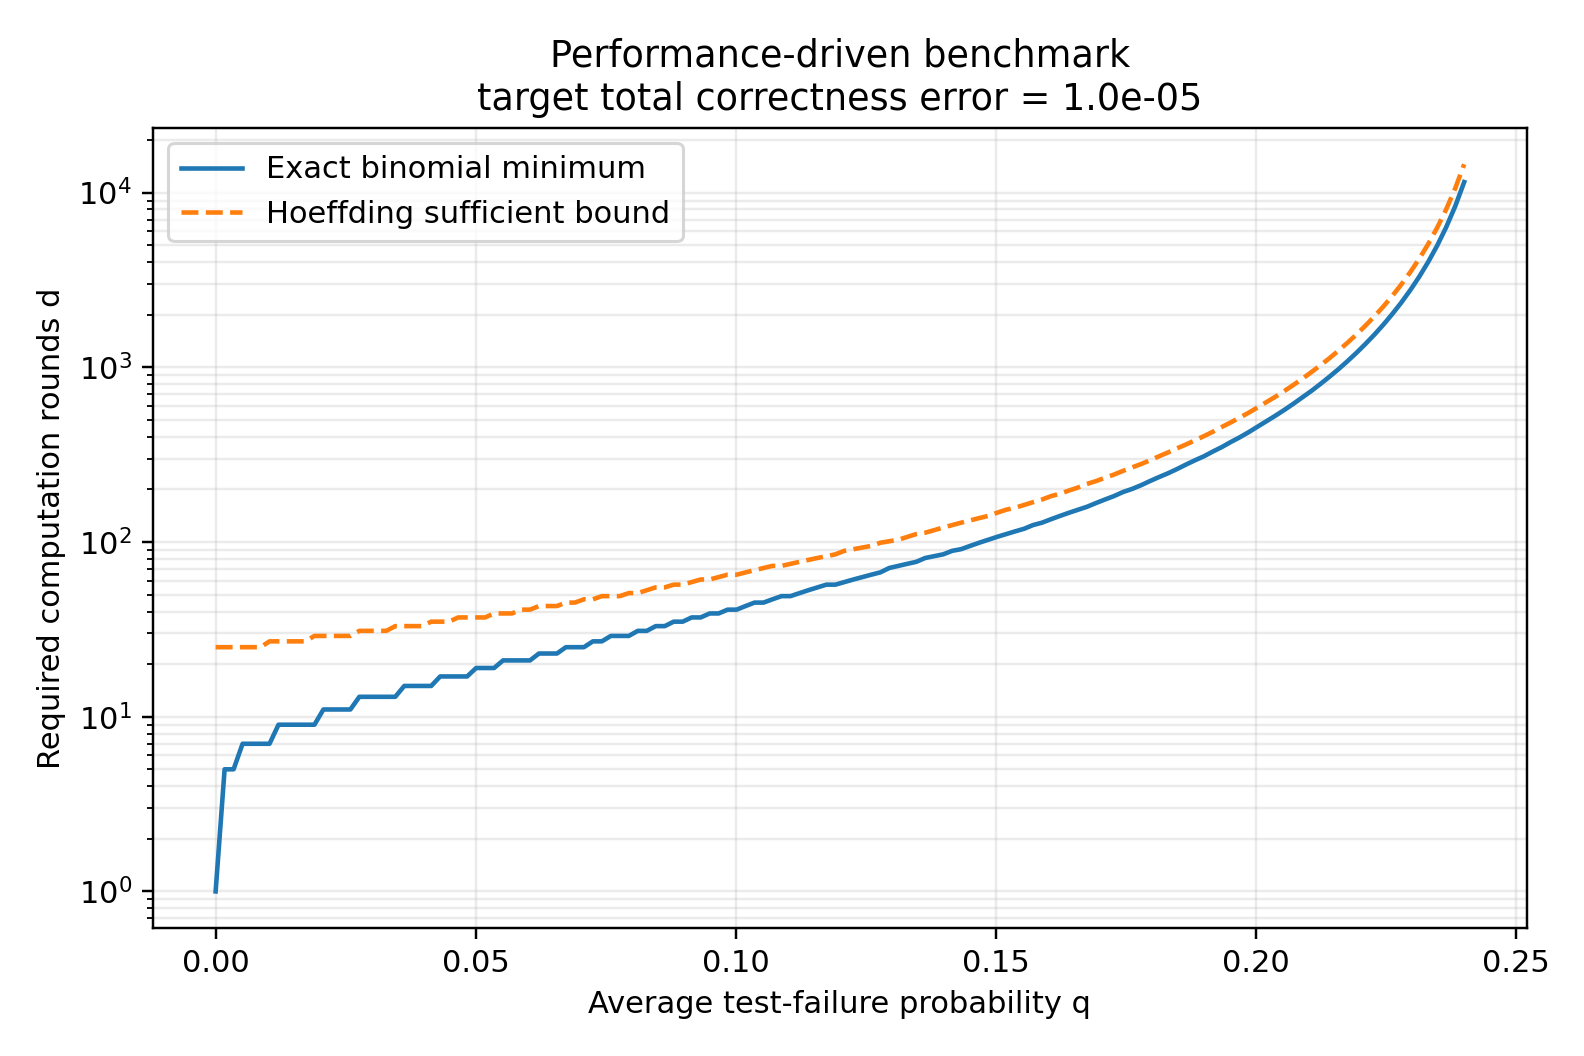
\includegraphics[width=0.82\linewidth]{figures/performance_fixed_epsilon.png}
\caption{Performance-driven benchmark generated by the accompanying script for
$k=2$, $c=0$, $\eps_\star=10^{-5}$, and
$\eps_{\mathrm{bench}}=10^{-6}$. The exact binomial calculation is compared
with the sufficient Hoeffding bound.}
\label{fig:performance}
\end{figure}

\section{Cost-driven benchmark}

Fix an odd computation-round budget $d_0$. For each circuit dimension $\ell$,
Equation~\eqref{eq:exact-tail} gives the exact achieved correctness error
\begin{equation}
  \eps_{\mathrm{tot}}^{\mathrm{exact}}(\ell;d_0)
  \le \eps_{\mathrm{bench}}
  +\eps_{\mathrm{vote}}^{\mathrm{exact}}
  (d_0,p_\ell^{\mathrm U}).
  \label{eq:cost-exact}
\end{equation}
The analytic upper bound is
\begin{equation}
  \eps_{\mathrm{tot}}^{\mathrm H}(\ell;d_0)
  \le \eps_{\mathrm{bench}}
  +\exp\!\left[-2d_0
    \left(\frac12-p_\ell^{\mathrm U}\right)^2
  \right].
  \label{eq:cost-hoeffding}
\end{equation}
This is the cost-driven map
\begin{equation}
  p_{\mathrm{err}}\longmapsto\eps_{\mathrm{tot}}
  \qquad\text{at fixed }d_0.
\end{equation}

\begin{figure}[ht]
\centering
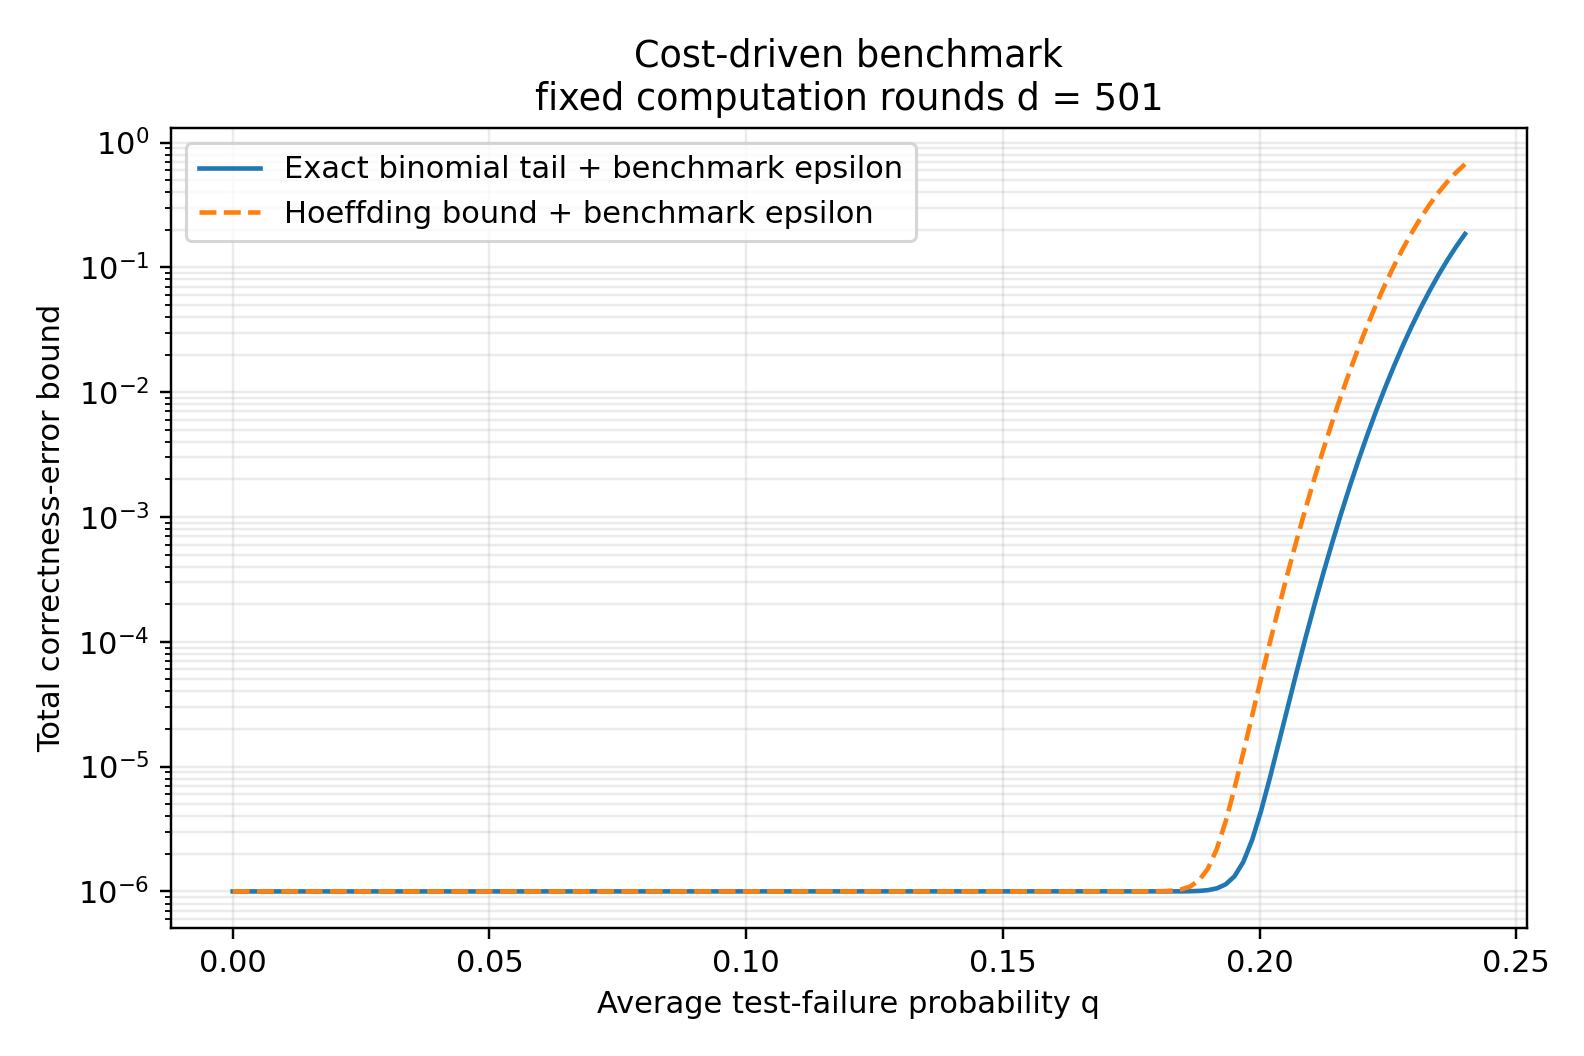
\includegraphics[width=0.82\linewidth]{figures/cost_fixed_rounds.png}
\caption{Cost-driven benchmark generated for a fixed budget $d_0=501$. The
benchmark confidence error creates a floor at
$\eps_{\mathrm{bench}}=10^{-6}$.}
\label{fig:cost}
\end{figure}

\section{Circuit-dimension maps and heatmaps}

Circuit dimension does not enter the majority-vote equations directly. It
enters through the experimentally measured noise:
\begin{equation}
  \ell
  \longmapsto q_\ell^{\mathrm U}
  \longmapsto p_\ell^{\mathrm U}
  \longmapsto
  \begin{cases}
    d_{\min}(\ell;\eps_\star), & \text{performance-driven},\\
    \eps_{\mathrm{tot}}(\ell;d_0), & \text{cost-driven}.
  \end{cases}
  \label{eq:dimension-pipeline}
\end{equation}
For a scalar dimension $\ell$, the script generates line plots. For circuits
indexed by width and depth, it generates three heatmaps: the upper confidence
bound on circuit-level noise, the required number of computation rounds at
fixed $\eps_\star$, and the achieved correctness error at fixed $d_0$.

\begin{figure}[ht]
\centering
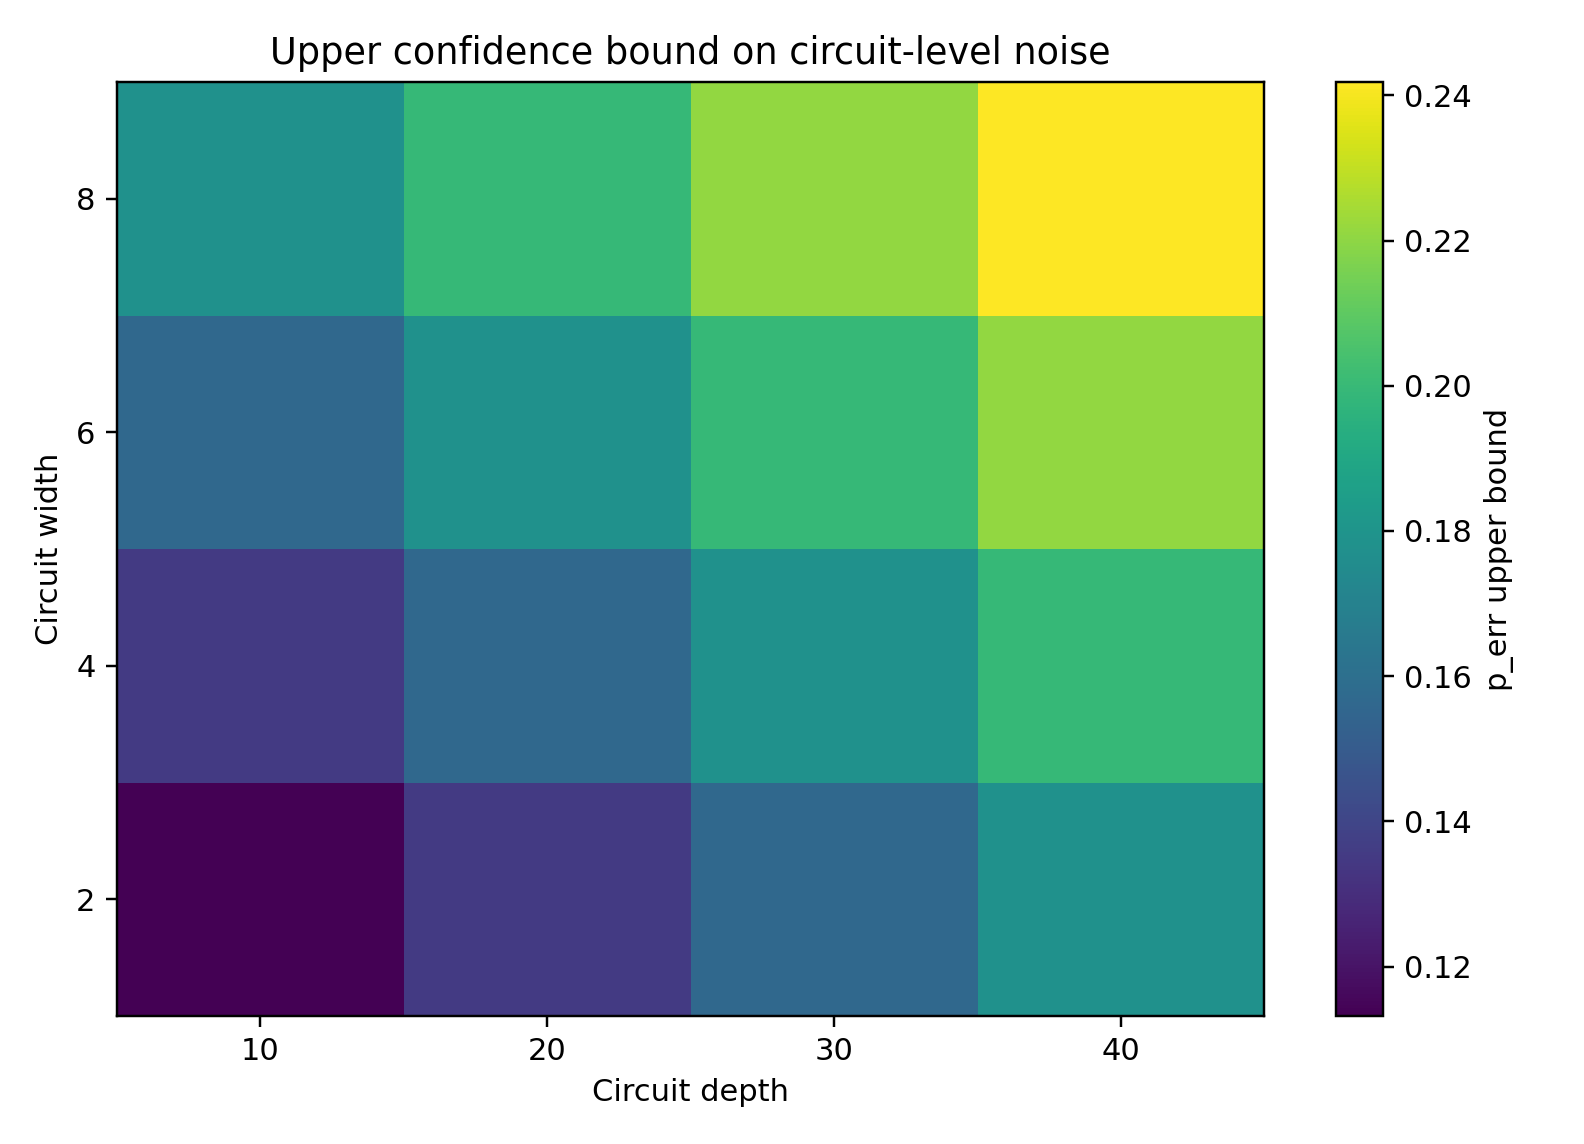
\includegraphics[width=0.78\linewidth]{figures/heatmap_noise_upper.png}
\caption{Example upper-confidence noise map over circuit width and depth. The
example data are synthetic and are included only to demonstrate the workflow.}
\label{fig:noise-heatmap}
\end{figure}

\begin{figure}[ht]
\centering
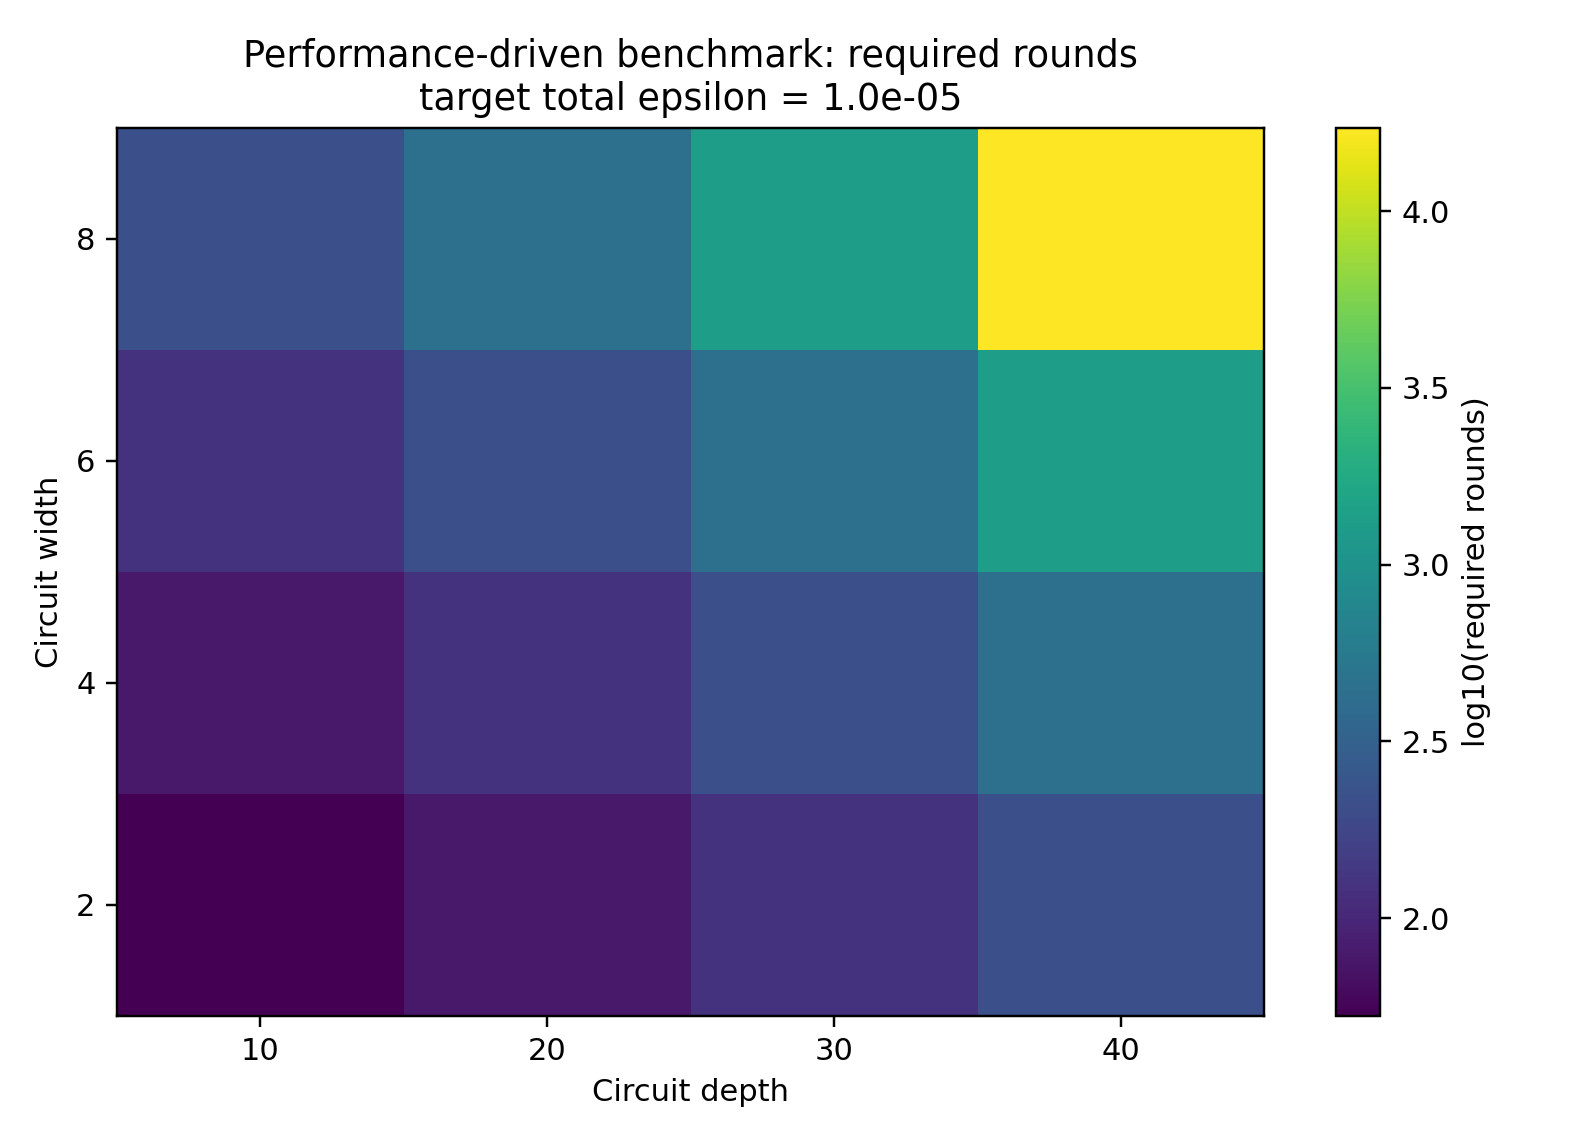
\includegraphics[width=0.78\linewidth]{figures/heatmap_required_rounds.png}
\caption{Performance-driven heatmap obtained by applying
Equation~\eqref{eq:dmin-exact} to every circuit instance. The color scale is
logarithmic in the required number of rounds.}
\label{fig:rounds-heatmap}
\end{figure}

\begin{figure}[ht]
\centering
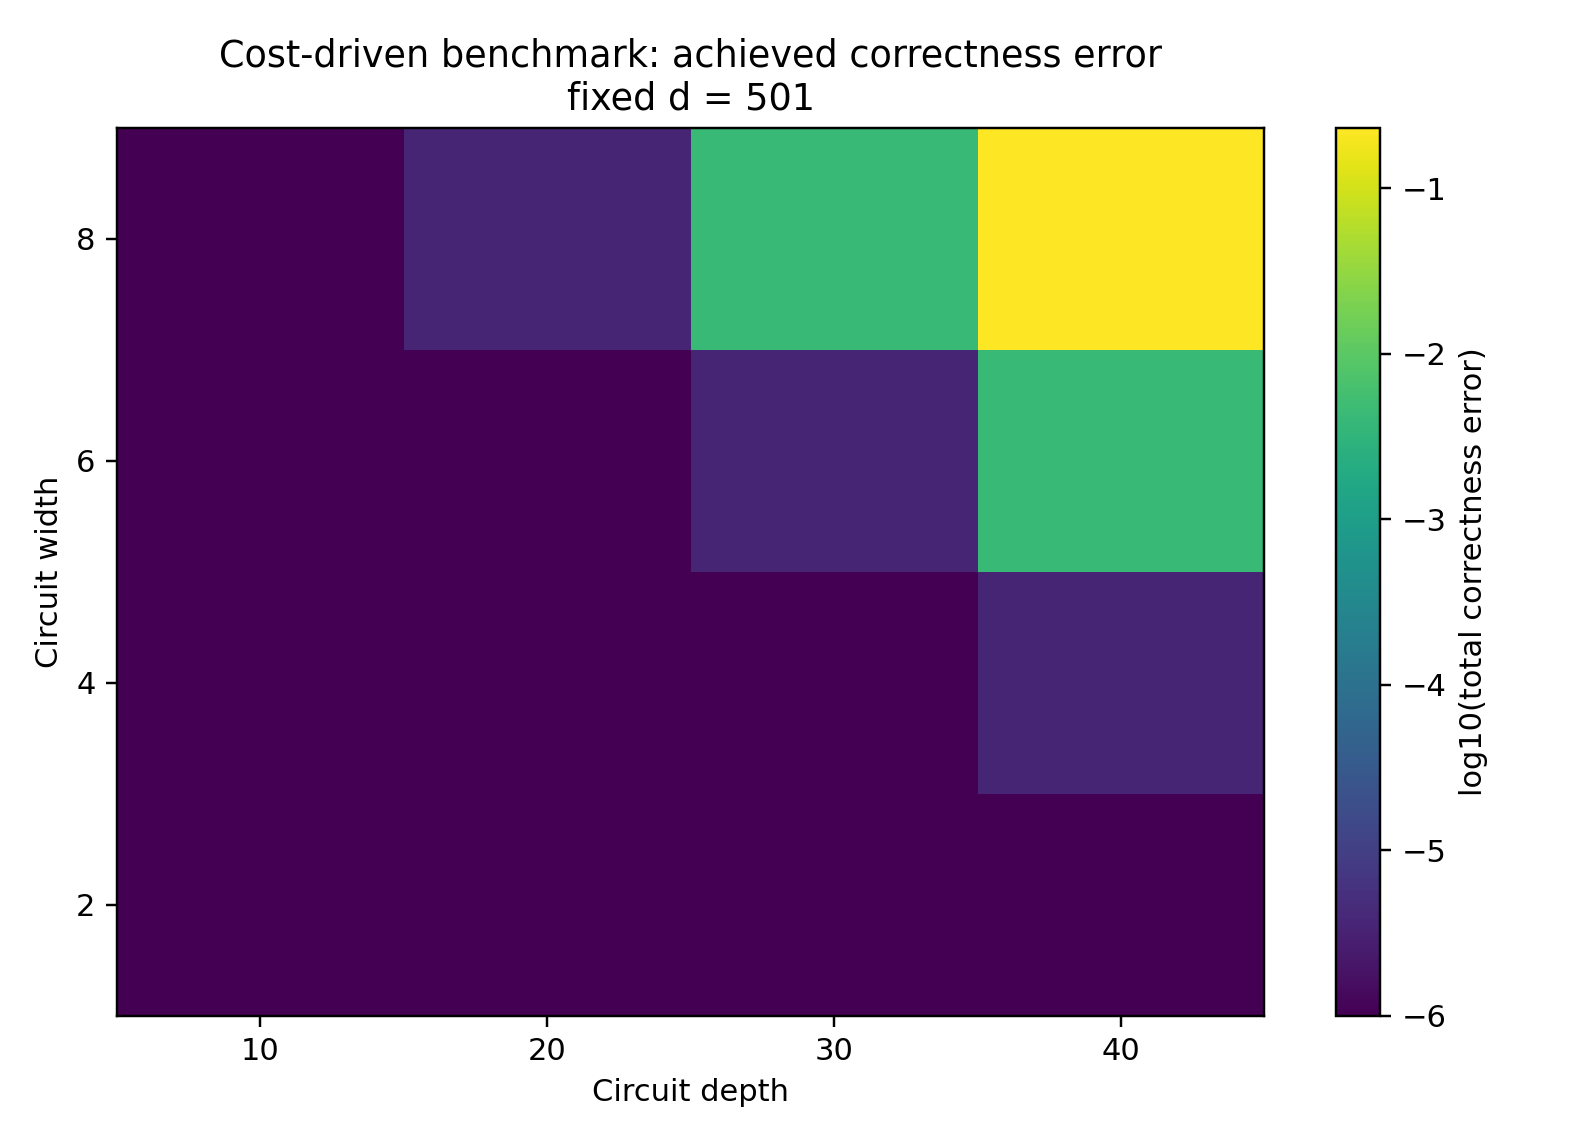
\includegraphics[width=0.78\linewidth]{figures/heatmap_achieved_epsilon.png}
\caption{Cost-driven heatmap obtained by applying
Equation~\eqref{eq:cost-exact} at fixed $d_0=501$. The color scale is
logarithmic in the correctness-error bound.}
\label{fig:epsilon-heatmap}
\end{figure}

\section{The $1/4$ threshold for two test types}

For $k=2$ and $c=0$, Equation~\eqref{eq:p-upper} becomes
\begin{equation}
  p_\ell^{\mathrm U}=2q_\ell^{\mathrm U}.
\end{equation}
Majority amplification requires $p_\ell^{\mathrm U}<1/2$, hence
\begin{equation}
  q_\ell^{\mathrm U}<\frac14.
  \label{eq:quarter-threshold}
\end{equation}
More generally, Equations~\eqref{eq:alpha} and \eqref{eq:p-upper} give
\begin{equation}
  q_\ell^{\mathrm U}<\frac{\alpha}{k}
  =\frac{1-2c_\ell}{k(2-2c_\ell)}.
\end{equation}
The relevant quantity is the upper confidence bound $q_\ell^{\mathrm U}$, not
only the observed frequency $\widehat q_\ell$. As
$q_\ell^{\mathrm U}\uparrow1/4$, the denominator in
Equation~\eqref{eq:dmin-hoeffding} tends to zero and the required number of
computation rounds diverges. Thus $1/4$ is an asymptotic boundary in the
conservative model, not a practical operating point.

\section{Connection with the structure of the proof}

The reformulation uses three ingredients from the verification analysis:

\begin{enumerate}[leftmargin=2em]
  \item \textbf{Correctness.} The paper bounds the probability that a majority
  of $d$ honest computation rounds is wrong by
  $\exp[-2d(1/2-c)^2]$. The benchmarked version replaces $c$ by the
  data-dependent upper bound $p_\ell^{\mathrm U}$.

  \item \textbf{Trap detection.} The security argument ensures that a harmful
  deviation is detected by at least one of the $k$ trap types. This yields the
  conservative conversion $r_\ell\le kq_\ell$.

  \item \textbf{Robustness.} The paper treats noisy test failures through a
  concentration argument and requires the honest noise rate to lie below the
  accepted test threshold. In the i.i.d. benchmark, the threshold is replaced
  by a confidence interval inferred from a dedicated test block.
\end{enumerate}

The malicious proof must retain a hidden random partition and maximize over
correlated attacks. The present benchmark does neither: it estimates one fixed
stationary parameter and extrapolates it to later computation rounds.

\section{Recommended experimental workflow}

\noindent\fbox{%
\begin{minipage}{0.94\linewidth}
\textbf{Input:} a circuit instance $\ell$, number of tests $s_\ell$, target
confidence failure $\eps_{\mathrm{bench}}$, test count $Y_\ell$, number of test
types $k$, intrinsic ideal error $c_\ell$, and either a target error
$\eps_\star$ or a fixed computation budget $d_0$.

\medskip
\textbf{Step 1.} Compute $\widehat q_\ell=Y_\ell/s_\ell$ and a one-sided upper
confidence bound $q_\ell^{\mathrm U}$.

\textbf{Step 2.} Convert it to
$p_\ell^{\mathrm U}=c_\ell+(1-c_\ell)\min\{1,kq_\ell^{\mathrm U}\}$, unless a
tighter project-specific transfer function is available.

\textbf{Step 3a, performance-driven.} Find the smallest odd $d$ satisfying
Equation~\eqref{eq:dmin-exact}.

\textbf{Step 3b, cost-driven.} Evaluate Equation~\eqref{eq:cost-exact} at the
available odd budget $d_0$.

\textbf{Output:} for every circuit dimension, report
$(\widehat q_\ell,q_\ell^{\mathrm U},p_\ell^{\mathrm U},d_{\min},
\eps_{\mathrm{tot}}(d_0))$.
\end{minipage}}

\section{Limitations}

The conclusions depend on stationarity, independence, and the test-to-computation
transfer inequality. Correlated noise, drift between the benchmark block and
the computation block, adaptive behavior, or circuit-dependent changes not
captured by the selected dimension invalidate the simple binomial model. A
practical implementation should therefore record time order, repeat benchmark
blocks periodically, and test for drift or overdispersion before interpreting
the resulting curves as correctness guarantees.

\section{Software}

The accompanying file \texttt{iid\_benchmark\_plots.py} implements:

\begin{itemize}[leftmargin=2em]
  \item exact and Hoeffding majority-vote calculations;
  \item one-sided Clopper--Pearson and Hoeffding confidence bounds;
  \item the three meanings of \texttt{p\_err} described in Section~3;
  \item performance- and cost-driven plots;
  \item one-dimensional circuit-family plots;
  \item width/depth heatmaps and a derived CSV summary.
\end{itemize}

\begin{thebibliography}{1}
\bibitem{sater2026magicblindness}
S.~A. Sater and H.~Ollivier.
\newblock Composable Verification in the Circuit-Model via Magic-Blindness.
\newblock arXiv:2601.07111v2, 2026.
\end{thebibliography}

\end{document}
